\subsection{Zapora bezstanowa}
\label{sec:bezstanowe}


\subsubsection{Opis zadania}

Zadanie z pierwszej części ćwiczenia polegało na konfiguracji zapory
odrzucającej przychodzące połączenia \ssh{} z maszyny \volt{} na dodatkowy
interfejs maszyny \kdwa. Zadanie zrealizowano korzystając z \ipfw{} oraz \pf.

Na maszynie \kdwa{} uruchomiono i skonfigurowano dodatkowy interfejs \emo{} z
adresem IP \emoip. Wykorzystane połączenia między maszynami \volt{} i \kdwa{} są
przedstawione na schemacie \ref{fig:bezstanowe:polaczenia}.

%TODO machnij schemat pls, bo masz ładniejszy program i mniej roboty niż dia > pdf

% k1% ifconfig
% vr0: flags=8843<UP,BROADCAST,RUNNING,SIMPLEX,MULTICAST> metric 0 mtu 1500
%         options=82808<VLAN_MTU,WOL_UCAST,WOL_MAGIC,LINKSTATE>
%         ether 00:40:63:de:28:a9
%         inet 194.29.146.247 netmask 255.255.255.0 broadcast 194.29.146.255
%         media: Ethernet autoselect (100baseTX <full-duplex>)
%         status: active
% ipfw0: flags=8801<UP,SIMPLEX,MULTICAST> metric 0 mtu 65536
% lo0: flags=8049<UP,LOOPBACK,RUNNING,MULTICAST> metric 0 mtu 16384
%         options=3<RXCSUM,TXCSUM>
%         inet 127.0.0.1 netmask 255.0.0.0
% em0: flags=8843<UP,BROADCAST,RUNNING,SIMPLEX,MULTICAST> metric 0 mtu 1500
%         options=209b<RXCSUM,TXCSUM,VLAN_MTU,VLAN_HWTAGGING,VLAN_HWCSUM,WOL_MAGIC>
%         ether 00:1b:21:07:c9:8e
%         inet 10.146.226.128 netmask 255.255.0.0 broadcast 10.146.255.255
%         media: Ethernet autoselect (1000baseT <full-duplex>)
%         status: active

\begin{figure}[h!]
  \centering
  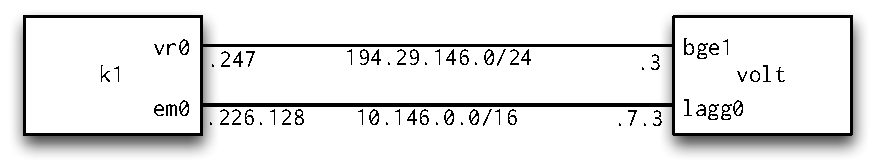
\includegraphics[width=12cm]{figury/bezstanowe/polaczenia.pdf}
  \caption{Schemat połączeń wykorzystanych przy realizacji pierwszej części ćwiczenia.}
  \label{fig:bezstanowe:polaczenia}
\end{figure}


\subsubsection{Wykonanie --- \pf}
\label{bezstanowa:pf}

Ogólna składnia reguły w konfiguracji \pf{} jest następująca:

\begin{lstlisting}
akcja [kierunek] [log] [quick] [on interface] [af] [proto protocol] \
   [from src_addr [port src_port]] [to dst_addr [port dst_port]] \
   [flags tcp_flags] [state]
\end{lstlisting}

Jednocześnie składnia pliku konfiguracyjnego \pf{} pozwala przypisywać
symboliczne nazwy zmiennym, co zwiększa jego czytelność.

Po zapoznaniu się ze składnią reguł sprawdzono, że połączenie \ssh{} z maszyny
\volt{} na adres \emoip{} jest możliwe. Następnie skonfigurowano zaporę \pf{} w
tworząc regułę:

\begin{lstlisting}[label=bezstanowe:pf.conf]
#/etc/pf.conf
drugi_interfejs = "em0"
volt = "10.146.7.3"
block in quick on $drugi_interfejs proto {tcp udp} from $volt to any port ssh
\end{lstlisting}

\noindent Całe zadanie realizuje reguła z ostatniej linii listingu
\ref{bezstanowe:pf.conf}:

\begin{description}

\item[\texttt{akcja}\textnormal{,}] którą wybraliśmy to \texttt{block}. Pakiet,
do którego zostanie zastosowana akcja \texttt{block} zostanie odrzucony.
Zależnie od konfiguracji zapora może także przesłać nadawcy informację o tym, że
jego pakiet nie osiągnął celu. Zależnie od protokołu, odpowiedzią będzie pakiet
\texttt{TCP RST} -- dla połączenia \tcp{} albo \texttt{ICMP Unreachable} -- w
przypadku pozostałych typów połączeń.

\item[\texttt{kierunek}] w naszym przypadku \texttt{in} oznacza, że reguła
dotyczy połączeń przychodzących.

\item[\texttt{quick}] oznacza, że \texttt{akcja} powinna być wykonana
natychmiast. W \pf{} inaczej niż w \ipfw{} pakiet może zostać dopasowany do
wielu reguł. Reguły dopasowywane są według ich kolejności w pliku
konfiguracyjnym --- od góry do dołu.

\item[\texttt{on}] przyjmuje nazwę interfejsu, którego ruch chcemy filtrować.

\item[\texttt{proto}] przyjmuje dowolną nazwą protokołu zadeklarowanego w pliku
\texttt{/etc/protocols}. Warto zwrócić uwagę na konstrukcję \texttt{\{udp tcp\}}
--- jest to lista. Reguła zawierająca listę zostaje podczas wczytywania pliku
konfiguracyjnego przepisana na wiele reguł. W pamięci tworzone są reguły dla
każdego elementu należącego do iloczynu kartezjańskiego wszystkich list
pierwotnej reguły.

\item[\texttt{from / to}] są informacją o adresie nadawcy i~odbiorcy.

\item[\texttt{port}] na końcu reguły określa, że blokowane mają być połączenia
przychodzące na port \ssh{}. Określenie numeru portu odpowiadającego \ssh{}
odbywa się na podstawie informacji w pliku \texttt{/etc/services}.

\end{description}

\pf{} wykonuje akcję z pierwszej napotkanej reguły z dyrektywą \texttt{quick}.
Jeżeli żadna reguła nie ma takiej dyrektywy, to zostanie zastosowana akcja z
ostatniej dopasowanej reguły. Po uruchomieniu zapory nie udało się nawiązać
połączenia \ssh{} z maszyny \volt{} na \emoip{}, co było oczekiwanym rezultatem.


\subsubsection{Wykonanie --- \ipfw{}}
\label{bezstanowa:ipfw}

\ipfw{} w przeciwieństwie do \pf{} nie posiada własnej składni plików
konfiguracyjnych. Zamiast tego regułami filtrowania zarządza się korzystając z
polecenia \texttt{ipfw}. Polecenie to pozwala na modyfikowanie zestawu reguł z
poziomu jednej reguły. Pozwala to łatwo tworzyć dynamiczne zestawy reguł.
Wystarczy połączyć polecenie \ipfw{} i \cron{} aby uzyskać regułę zależną od
godziny.

Rozwiązanie takie nie oznacza, że język konfiguracyjny jest ubogi w stosunku do
\pf{}. Co prawda samo polecenie \ipfw{} nie obsługuje zmiennych, ale za to
możliwe jest korzystanie ze zmiennych powłoki. Możliwe jest także używanie
konstrukcji warunkowych czy pętli, co pozwala na tworzenie zaawansowanych i
dynamicznych zestawów reguł bez potrzeby przeładowywania całej konfiguracji
zapory.

\begin{lstlisting}
k2$ sudo ipfw add 100 deny tcp from 10.146.7.3 to any dst-port 22 via em0
k2$ sudo ipfw add 200 deny udp from 10.146.7.3 to any dst-port 22 via em0
\end{lstlisting}

Składnia polecenia jest dość podobna, do tego co zostało opisane w sekcji
\ref{bezstanowa:pf}. Po komendzie \texttt{add} podawany jest numer reguły, która
ma zostać utworzona. Podobnie jak w \pf{} reguły o niższym numerze mają wyższy
priorytet od reguł z numerami niższymi. W przeciwieństwie do \pf{} akcja jest
wykonywana od razu po znalezieniu pasującej reguły.


\subsubsection{Filtrowanie przed ustanowieniem połączenia}

Teoretycznie, w protokole \tcp{}, aby zablokować cały ruch wystarczy zablokować
możliwość ustanowienia połączenia. Można więc dodać do zapory następującą
regułę:

\begin{lstlisting}
l2% sudo ipfw add 100 deny tcp from 10.146.7.3 to any dst-port 22 via em0 tcpflags syn
\end{lstlisting}

Reguła ta sprawi, że zostaną odrzucone wszystkie przychodzące pakiety z flagą
\texttt{SYN}. Jeżeli celem jest wyłącznie zablokowanie ruchu, naszym zdaniem
lepiej stosować rozwiązanie z sekcji \ref{bezstanowa:pf}. Reguła zastosowana w
tamtej sekcji powinna działać wydajniej, ponieważ nie musi analizować flag
\tcp{} każdego pakietu.

Ponadto reguła z sekcji \ref{bezstanowa:pf} zablokuje też już nawiązane
połączenia i komunikację nie będącą częścią połączeń takie jak błędnie wysłane
pakiety, czy próby ataku na stos \texttt{TCP/IP} systemu za firewallem.
Stosowanie filtrowania opartego na flagach \tcp{} ma sens, jeżeli celem jest
zezwolenie na połączenie pomiędzy dwoma maszynami tylko jeśli jedna z nich jest
maszyną inicjującą połączenie.

Rozważmy regułę bez podanego portu:

\begin{lstlisting}
k2% sudo ipfw add 300 deny tcp from 10.146.7.3 to any via em0 tcpflags syn
\end{lstlisting}

Reguła taka pozwoli na komunikację z maszyną \volt{} za pomocą \tcp{} wtedy i
tylko wtedy, gdy maszyna \volt{} nie jest maszyną inicjującą połączenie. Takie
rozwiązanie jest analogiczne do reguł stanowych, natomiast nie zużywa pamięci na
przechowywanie informacji o tym, które połączenia zostały otwarte przez którą ze
stron połączenia.
